\documentclass[a4paper,11pt,danish,titlepage]{article}

\usepackage[latin1]{inputenc}
\usepackage[T1]{fontenc}
\usepackage[danish]{babel}
\usepackage{url}
\usepackage{lastpage}
\usepackage{bookmark}
\usepackage{fancyhdr}
\usepackage{graphicx}
\usepackage[all]{xy}
\usepackage{sectsty}
\usepackage{amsmath}

\usepackage{parskip}

\usepackage{charter}
\usepackage{cmbright}
\renewcommand{\familydefault}{\rmdefault}
\allsectionsfont{\sffamily}

\date{Januar 2010}

\newcommand{\thetitle}{Computergrafik}

\newcommand{\email}[1]{\href{mailto:#1}{\texttt{#1}}}

\title{{\huge DTU 02651} \\ {\normalsize \thetitle}}

\author{
  {\small
    \begin{tabular}{llll}
      Julian M�ller & 180387-1619 & s084246 & \email{boolean@diku.dk} \\
      Steen Nordsmark Pedersen & 150287-1435 & s092642 & \email{acid@diku.dk} \\
    \end{tabular}
  }
}

\numberwithin{figure}{subsection}

\begin{document}

\maketitle

\pagestyle{fancy}
	\lhead{\thetitle}
	\chead{}
	\rhead{DTU, efter�r 2009}
	\lfoot{}
	\cfoot{\thepage}
	\rfoot{}
\setcounter{page}{1}
\pagenumbering{roman}

\tableofcontents
\newpage

\listoffigures

Figurerne er nummereret p� f�lgende m�de:

\texttt{<ugeopgavenummer>.<delopgavenummer>.<figurnummer>}

Dvs. at figuren \emph{1.2.1} er den f�rste figur, tilh�rende den anden
delopgave i den f�rste ugeopgave.
\newpage

\pagestyle{fancy}
	\lhead{\thetitle}
	\chead{}
	\rhead{DTU, efter�r 2009}
	\lfoot{}
	\cfoot{Side \thepage \ af \pageref{LastPage}}
	\rfoot{}
\setcounter{page}{1}
\pagenumbering{arabic}

\chapter{Ugeopgave 1}
\label{sec:ugeopgave-1}

Form�let med denne opgave var at blive introduceret til at lave,
redigere, linke og k�re C- og C++-programmer, der er bruger OpenGL,
GLU og GLUT.

\section{Del 1}
\label{sec:del-1}

Programmet, n�r det k�res, viser vinduet i figur \ref{fig:1-1-1}.

\begin{figure}[hp]
\centering
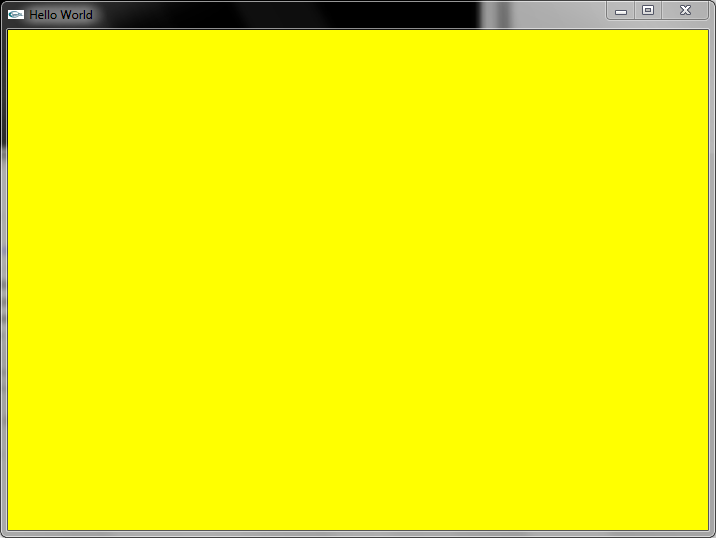
\includegraphics[width=8cm]{../exercise1/part1/screenshots/part1_1.png}
\caption{F�rste k�rsel}
\label{fig:1-1-1}
\end{figure}

N�r der tilf�jes de udkommenterede linjer, bliver koordinatsystemet
sat, s� man kan se den gule polygon i sin fulde udstr�kning p�
sk�rmen. Det kan ses p� figur \ref{fig:1-1-2}.

\begin{figure}[hp]
\centering
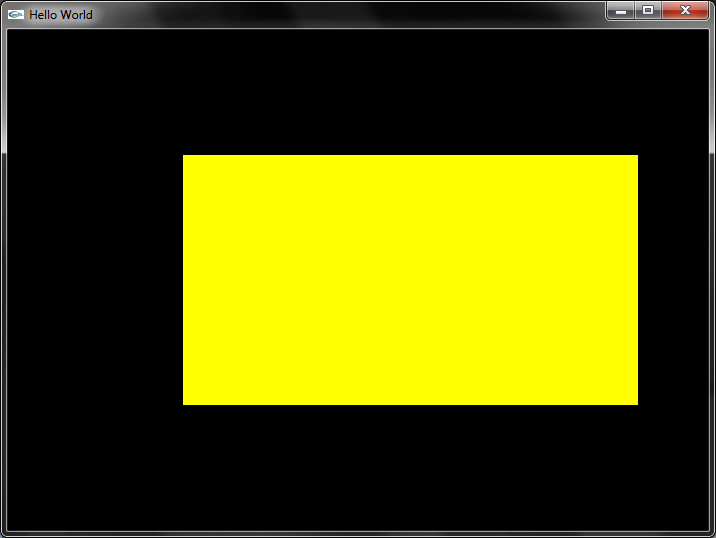
\includegraphics[width=8cm]{../exercise1/part1/screenshots/part1_2.png}
\caption{Tilf�jelse af udkommenterede linjer}
\label{fig:1-1-2}
\end{figure}

\section{Del 2}
\label{sec:del-2}

Programmet, n�r det k�res, viser vinduet i figur \ref{fig:1-2-1}.
%
Dern�st blev der tilf�jet en r�d trekant, med knuderne $(2,2)$,
$(5,2)$ og $3.5,5)$. Dette kan ses p� figur \ref{fig:1-2-2}.
%
Trekanten er herefter translateret med vektoren $(6,7)$. Det ses p�
figur \ref{fig:1-2-3}.
%
Efterf�lgende er de enkelte hj�rner i trekanten blevet farve
henholdsvis r�d, gr�n og bl�. Det ses p� figur \ref{fig:1-2-4}.
%
Rektanglet er herefter blevet roteret 45 grader mod uret om sin egen
midte. Dette er gjort ved at translatere rektanglet, s� dets midte var
i $(0,0)$ og derefter rotere om en akse. Resultatet ses p� figur \ref{fig:1-2-5}.

\begin{figure}[hp]
\centering
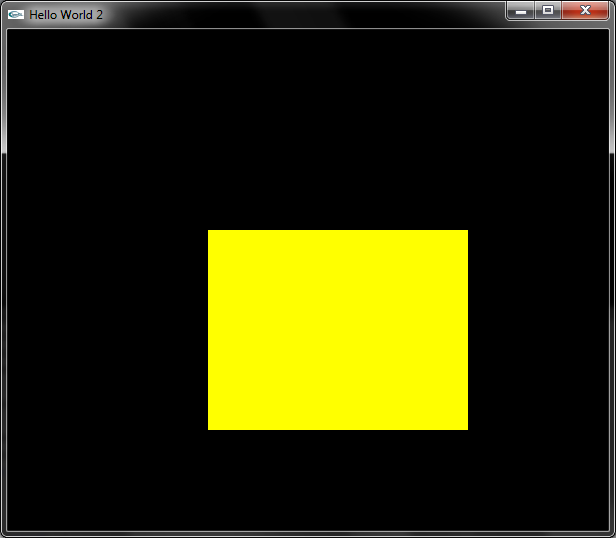
\includegraphics[width=8cm]{../exercise1/part2/screenshots/part2_1.png}
\caption{F�rste k�rsel}
\label{fig:1-2-1}
\end{figure}

\begin{figure}[hp]
\centering
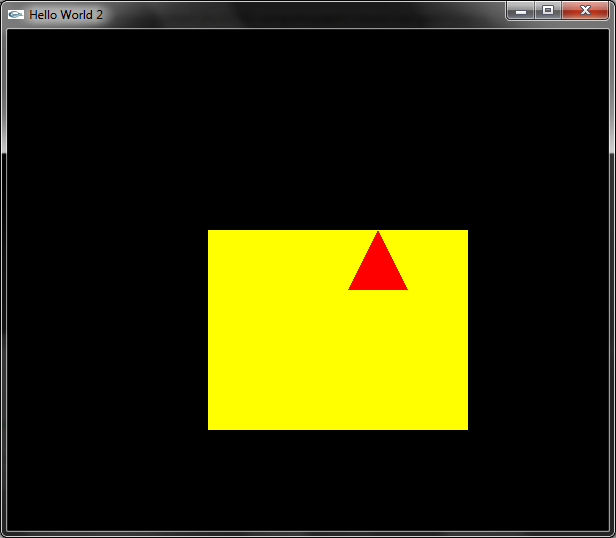
\includegraphics[width=8cm]{../exercise1/part2/screenshots/part2_2.png}
\caption{Tilf�jelse af en trekant}
\label{fig:1-2-2}
\end{figure}

\begin{figure}[hp]
\centering
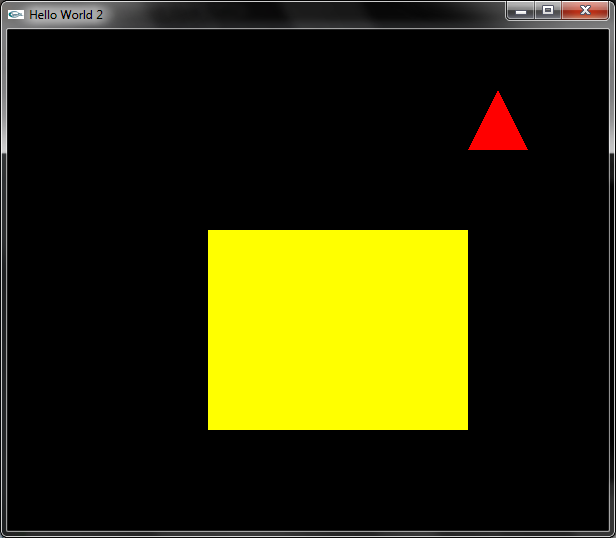
\includegraphics[width=8cm]{../exercise1/part2/screenshots/part2_3.png}
\caption{Translatering af trekant}
\label{fig:1-2-3}
\end{figure}

\begin{figure}[hp]
\centering
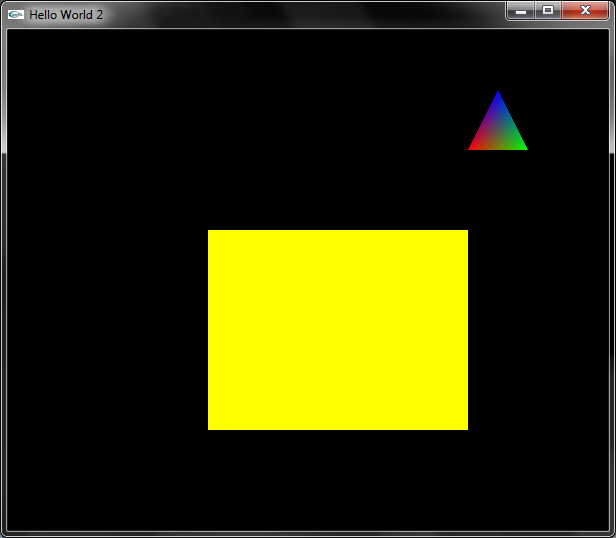
\includegraphics[width=8cm]{../exercise1/part2/screenshots/part2_4.png}
\caption{Omfarvning af trekant}
\label{fig:1-2-4}
\end{figure}

\begin{figure}[hp]
\centering
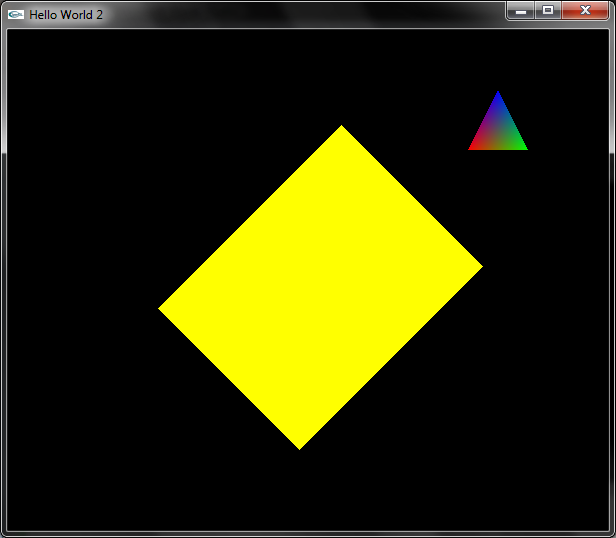
\includegraphics[width=8cm]{../exercise1/part2/screenshots/part2_5.png}
\caption{Rotering af rektangel}
\label{fig:1-2-5}
\end{figure}

\section{Del 3}
\label{sec:del-3}

K�rslen af dette program resulterede i figur \ref{fig:1-3-1}.

\begin{figure}[hp]
\centering
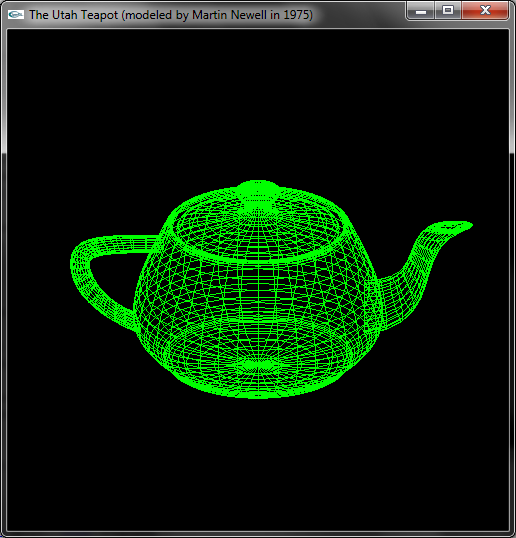
\includegraphics[width=8cm]{../exercise1/part3/screenshots/part3_1.png}
\caption{3D wireframe tepotte}
\label{fig:1-3-1}
\end{figure}

\section{Del 4}
\label{sec:del-4}

Vores genererede forside kan ses p� figur \ref{fig:1-4-1} (samt
naturligvis som forside p� dette dokument). De tre gr�nne cirkler
repr�senterer DIKUs farver og logo p� K�benhavns Universitet.

\begin{figure}[hp]
\centering
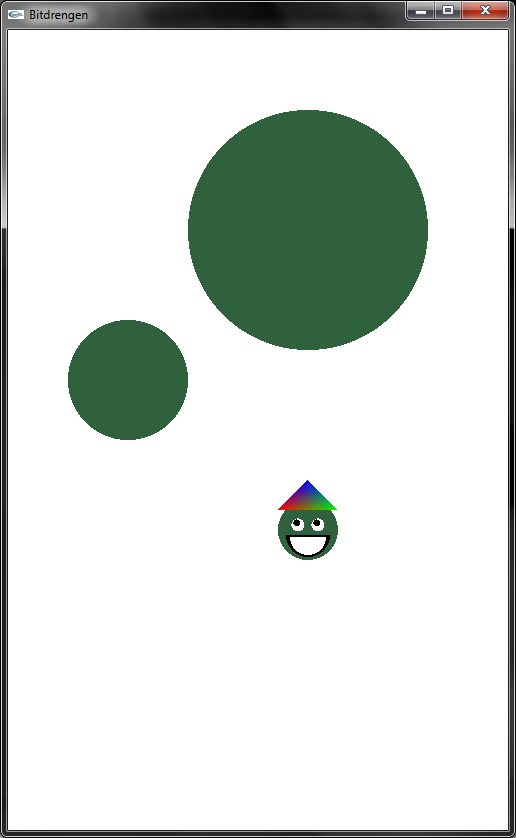
\includegraphics[width=8cm]{../exercise1/part4/screenshots/part4_1.png}
\caption{Projektforside}
\label{fig:1-4-1}
\end{figure}

\section{Del 5}
\label{sec:del-5}

I denne delopgave skulle vi tegne en cirkel. Til dette har vi brugt
\texttt{GL\_LINE\_LOOP} til at tegne 360 cirkelstykker, hvor
x- og y-koordinaterne er beregnet vha. hhv. $cos$ og $sin$. Til at
tegne en solid cirkel har vi lavet 360 trekanter, hvor de to hj�rner
er de samme som start- og slut-punkterne for linjestykkerne fra f�r og
det sidste hj�rne p� trekanten er cirklens centrum. Linjecirklen kan
ses p� figur \ref{fig:1-5-1} mens den udfyldte (og flerfarvede) cirkel
kan ses p� figur \ref{fig:1-5-2}.

\begin{figure}[hp]
\centering
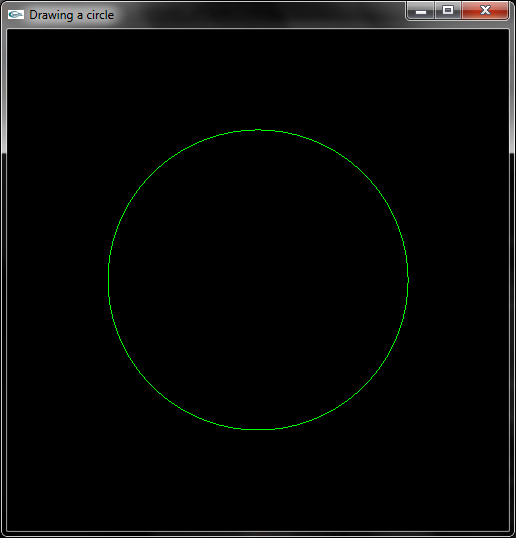
\includegraphics[width=8cm]{../exercise1/part5/screenshots/part5_1.png}
\caption{Linjecirkel}
\label{fig:1-5-1}
\end{figure}

\begin{figure}[hp]
\centering
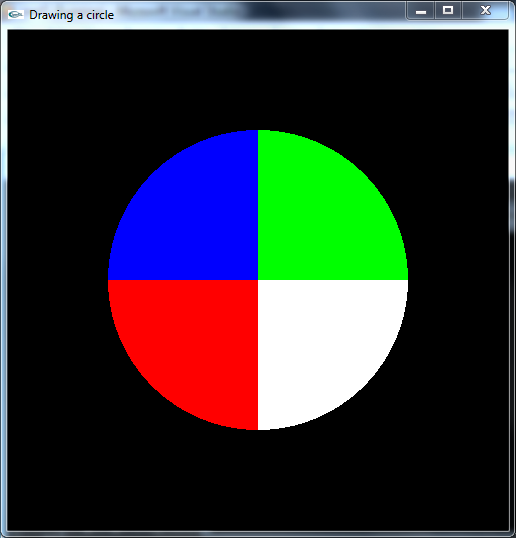
\includegraphics[width=8cm]{../exercise1/part5/screenshots/part5_2.png}
\caption{Udfyldt (flerfarvet) cirkel}
\label{fig:1-5-2}
\end{figure}

\section{Del 6}
\label{sec:del-6}

Vi har et \emph{window}/\emph{viewport}-par, der er defineret ved
koordinatparrene
%
\[
[(x_{wmin}, y_{wmin}),~ (x_{wmax}, y_{wmax})]
\]
%
samt
%
\[
[(x_{vmin}, y_{vmin}),~ (x_{vmax}, y_{vmax})]
\]
%
En transformation fra $(x_w, y_w)$ til $(x_v, y_v)$ kan defineres ved
de tre operationer:

\begin{itemize}
\item Translatering (til $(0,0)$)
\item Skalering
\item Translatering (tilbage)
\end{itemize}

Dermed er hele operationen, $M$, givet ved:
%
\begin{align*}
M = & T \left( x_{vmin},~y_{vmin} \right) \cdot \\
    & S \left(
        \dfrac{x_{vmax} - x_{vmin}}{x_{wmax} - x_{wmin}},~
        \dfrac{y_{vmax} - y_{vmin}}{y_{wmax} - y_{wmin}}
       \right)\cdot \\
    & T \left( x_{wmin},~y_{wmin} \right)
\end{align*}
%
Den sidste tranlatering er angivet f�rst, da man regner bagl�ns.

Matricerne for ovenst�ende, og det samlede resultat, $M$, vil dermed
v�re:

\begin{align*}
  M = & \begin{bmatrix}
          1 & 0 & x_{vmin} \\ 0 & 1 & y_{vmin} \\ 0 & 0 & 1
        \end{bmatrix} \cdot \\
      & \begin{bmatrix}
          \dfrac{x_{vmax} - x_{vmin}}{x_{wmax} - x_{wmin}} & 0 & 0 \\
          0 & \dfrac{y_{vmax} - y_{vmin}}{y_{wmax} - y_{wmin}} & 0 \\
          0 & 0 & 1 
        \end{bmatrix} \cdot \\
      & \begin{bmatrix}
          1 & 0 & -x_{wmin} \\
          0 & 1 & -y_{wmin} \\
          0 & 0 & 1
        \end{bmatrix} \\
    = & \begin{bmatrix}
          \dfrac{x_{vmax} - x_{vmin}}{x_{wmax} - x_{wmin}} & 0 &
          -x_{wmin} \cdot \dfrac{x_{vmax} - x_{vmin}}{x_{wmax} -
            x_{wmin}} + x_{vmin} \\
          0 & \dfrac{y_{vmax} - y_{vmin}}{y_{wmax} - y_{wmin}} &
          y_{wmin} \cdot \dfrac{y_{vmax} - y_{vmin}}{y_{wmax} -
            y_{wmin}} + y_{vmin} \\
          0 & 0 & 1
        \end{bmatrix}
\end{align*}

Multipliceres $M$ med et punkt $p$ med koordinaterne $(x,~y,~1)$ f�s
resultatet $p'$:

\begin{align*}
  p' = & M \cdot p \\
     = &
  \begin{bmatrix}
    \left(x - x_{wmin}\right) \cdot
    \frac{x_{vmax} - x_{vmin}}{x_{wmax} - x_{wmin}} + x_{vmin} &
    \left( y - y_{wmin} \right) \cdot
    \frac{y_{vmax} - y_{vmin}}{y_{wmax} - y_{wmin}} + y_{vmin} &
    1
  \end{bmatrix}
\end{align*}

\section{Del 7}
\label{sec:del-7}

K�rsel af programmet inden de �nskede operationer er udf�rt kan ses p�
figur \ref{fig:1-7-1}. Det kan her ses, at yw-aksen som yo-aksen ogs�
vender opad.

Vi har udf�rt de tre operationer i omvendt r�kkef�lge i OpenGL. Det
vil sige f�rst \texttt{glTranslate}, dern�st \texttt{glRotate} og til
sidst \texttt{glScale}. Med en skalering til dobbelt st�rrelse, har vi
forst�et dobbelt sidest�rrelse. Resultatet af dette, kan ses p� figur
\ref{fig:1-7-2}. Det kan her ses, at midten af terningen er i samme
h�jde som det �verste punkt i linjen fra $(1,0,0)$ til $(1,3,0)$.

Hvis operationerne blev udf�rt i den ``naturlige'' r�kkef�lge, var
resultatet som ses p� figur \ref{fig:1-7-3}, hvor man kan se at
translateringen ogs� er blevet skaleret med en faktor to.

\begin{figure}[hp]
\centering
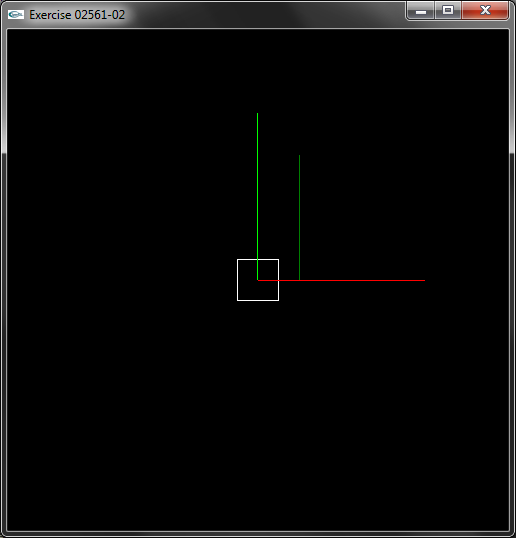
\includegraphics[width=8cm]{../exercise1/part7/screenshots/part7_1.png}
\caption{Uden transformationer}
\label{fig:1-7-1}
\end{figure}

\begin{figure}[hp]
\centering
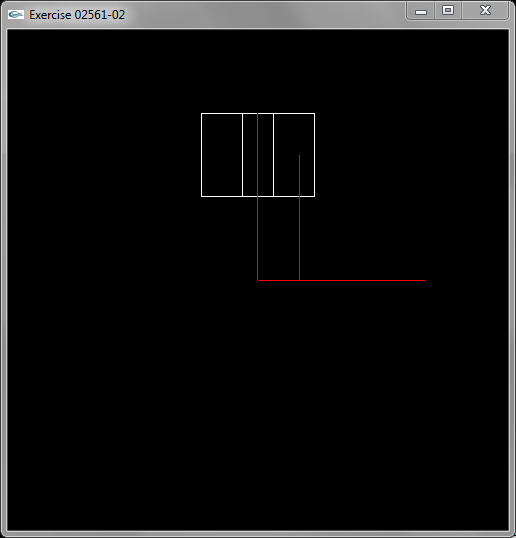
\includegraphics[width=8cm]{../exercise1/part7/screenshots/part7_2.png}
\caption{Enhedsterning: TRS}
\label{fig:1-7-2}
\end{figure}

\begin{figure}[hp]
\centering
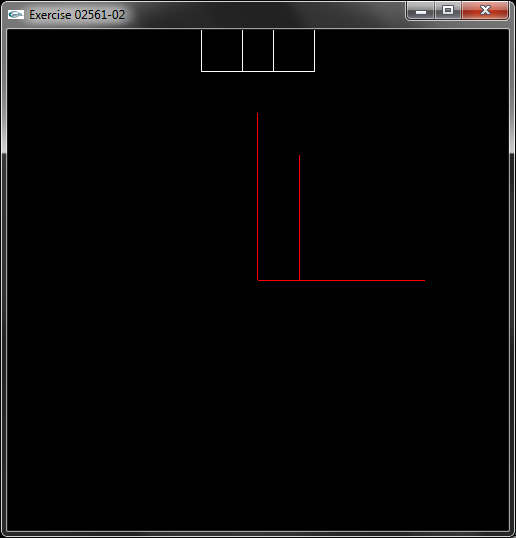
\includegraphics[width=8cm]{../exercise1/part7/screenshots/part7_3.png}
\caption{Enhedsterning: SRT}
\label{fig:1-7-3}
\end{figure}

\section{Del 8}
\label{sec:del-8}

Idet, der i denne opgave skal laves et front-perspektiv
(etpunktsperspektiv), viewplanet g�r igennem $(0,0,0)$ og kameraet er
placeret i $(20,5,5)$ kan \emph{at}-punktet fx v�re at finde i
$(20,5,-20)$, da et etpunksperspektiv har �t \emph{principal face} der
er parallel med viewplanet. \todo{omformuler (og overs�t?), s� det er
  mere klart}

For at f� en ordentligt billede af kassen, har vi valgt ogs� at lave
den med sidest�rrelse $2$ i stedet for $10$. Endvidere har vi lavet
kassen solid, med optegnede kanter, s� perspektiv og aksernes
placering er nemmere at vurdere. Frontperspektivet af kassen med
sidest�rrelse $10$ kan ses p� figur \ref{fig:1-8-1}, mens kassen med
sidest�rrelse $2$ kan ses p� figur \ref{fig:1-8-2}.

I stedet for at �ndre sidest�rrelsen, kunne vi for at f� et ordentligt
billede ogs� have translateret kassen til et andet punkt, eller
�ndret \emph{fov}-vinklen til fx. $90$. Det f�rste ville naturligvis
kunne give et billede af hele kassen ved at placere den l�ngere ude af
x-aksen samt under kameraet, mens en forst�rre�se af \emph{fov} ville
fungere som at zoome ud.

Den lille hvide prik p� begge billeder angiver forsvindingspunktet p�
horisonten for det brugte \emph{at}-punkt.

\begin{figure}[hp]
\centering
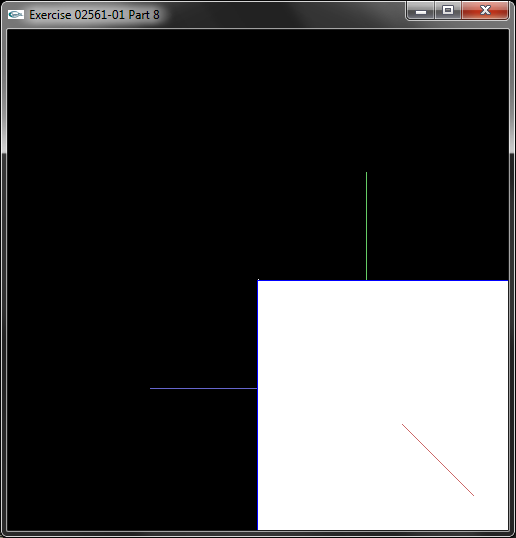
\includegraphics[width=8cm]{../exercise1/part8/screenshots/part8_1.png}
\caption{Frontperspektiv (sidest�rrelse: 10)}
\label{fig:1-8-1}
\end{figure}

\begin{figure}[hp]
\centering
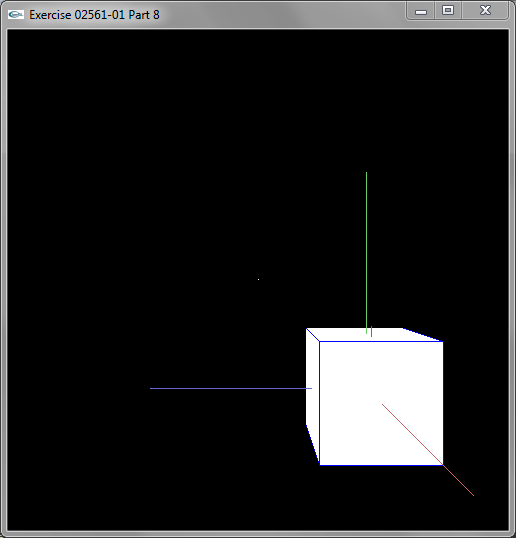
\includegraphics[width=8cm]{../exercise1/part8/screenshots/part8_2.png}
\caption{Frontperspektiv (sidest�rrelse: 2)}
\label{fig:1-8-2}
\end{figure}

Udover frontperspektivet, skulle der ogs� laves et X-perspektiv
(topunktsperspektiv). I et topunktsperspektiv er netop �n akse i
motivet parallel med viewplanet.


%%% Local Variables: 
%%% mode: latex
%%% TeX-master: "report_main"
%%% End: 

\end{document}

%%% Local Variables: 
%%% mode: latex
%%% TeX-master: "report_main"
%%% End: 